\documentclass[a4paper,10pt]{article}
\usepackage[utf8]{inputenc}
\usepackage{url}
\usepackage{amsmath}
\usepackage{graphicx}

%opening
\title{COMP417: Assignment 2\\Due Saturday, Feb 18 at 6pm}

\begin{document}

\maketitle

\section{A* implementation (5pts)}
Implement the A* algorithm for an omnidirectional robot on a 2D plane. You are given starter code
that implements Dijkstra's algorithm in Python at the following repository: \url{https://github.com/florianshkurti/comp417.git}, under the directory 
\path{comp417/path_planning_and_control_assignment/python}. You need to modify the function \path{plan()} in the file \path{astar_planner.py}.
You can run this file as follows:

  \path{cd} \path{path/to/comp417/path_planning_and_control_assignment/python/}
  
   \path{./astar_planner.py} \path{../worlds/map.pkl}

\noindent What you need to submit: 3 images of paths produced by your planner. Use the same starting state that is currently provided, and 
3 distinct destination states that are far from each other. Your images should be named \path{astar_result_[0|1|2]_firstname_lastname.png}

\section{RRT implementation (5pts)}
Implement the RRT algorithm for an omnidirectional robot on a 2D plane. You are given starter code
that implements some of the RRT functionality. You need to modify multiple functions which are annotated with TODOs in 
the file \path{rrt_planner.py}. Note that this version of the RRT is the simplest version to implement in the sense that we 
are not requiring kd-tree-based nearest neighbor queries and complicated collision queries. We use occupancy grids to simplify 
collision detection. Once you are done implementing the required functionality you can run this file as follows:

  \path{cd} \path{path/to/comp417/path_planning_and_control_assignment/python/}
 
  \path{./rrt_planner.py} \path{../worlds/map.pkl}

\noindent What you need to submit: 3 images of paths produced by your planner. Use the same starting state that is currently provided, and 
3 distinct destination states that are far from each other. Your images should be named \path{rrt_result_[0|1|2]_firstname_lastname.png}

\begin{figure}
  \begin{center}
    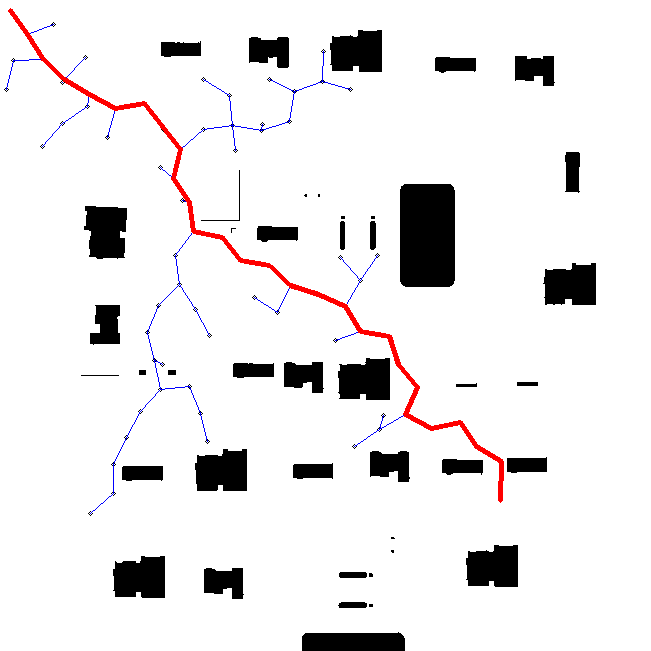
\includegraphics[width=0.4\textwidth]{rrt}
  \end{center}
  \caption{How the RRT planner will look like once you implement it}
\end{figure}

\section{LQR (2.5pts)}
Recall the example of the double integrator system with friction, or curling stone, that we saw in class:
\begin{equation}
m\ddot{\textbf{p}} = \textbf{u}-\alpha \dot{\textbf{p}} \nonumber
\end{equation}
\noindent where $\alpha$ is the friction coefficient, $\textbf{p}$ is the 2D position vector of the stone, and $\textbf{u}$ is the external control applied to the stone. 
You are given two curling stones of equal mass $m$. They start from different starting positions, with different starting velocities. You are tasked with finding an LQR 
controller/policy that receives feedback on the joint state of the two curling stones and outputs command vectors $\textbf{u}_1$ and $\textbf{u}_2$ so that the two stones 
end up very gently hitting each other and not bouncing away from each other. In other words, define a joint linear system 
\begin{equation}
  \textbf{x}_{t+1} = A\textbf{x}_t + B\textbf{u}_t
\end{equation}
\noindent and an instantaneous cost function
\begin{equation}
  g(\textbf{x}_t, \textbf{u}_t) = \textbf{x}^T_tQ\textbf{x}_t + \textbf{u}^T_tB\textbf{u}_t
\end{equation}
\noindent such that when the state $\textbf{x}_t$ stabilizes around $\textbf{0}$ the stones are touching each other and their individual velocities are also 
stabilized around $\textbf{0}$.

What you need to submit: a file called lqr.pdf with the definition of the matrices A, B, Q, R, as well as the steps you took to arrive at your formulation.    

\section{How to submit}
Similarly to assignment 1, you will submit all your work in a file called \path{path_planning_and_control_assignment.zip} which will contain
your extensions to the provided starter code, as well as the six images and the pdf file. 
\end{document}
